\documentclass[conference]{IEEEtran}
\usepackage{graphicx}

\usepackage{tikz}

\usepackage[colorlinks = true, citecolor = blue]{hyperref}

% math lib
\usepackage{amsmath}
\usepackage{mathrsfs}

% theorem
\usepackage{amsthm}
\theoremstyle{definition}
\newtheorem{lemma}{Lemma}
\newtheorem{theorem}{Theorem}
\newtheorem{assumption}{Assumption}
\newtheorem{corollary}{Corollary}
\newtheorem{problem}{Problem}
\newtheorem{definition}{Definition}

% operators
\DeclareMathOperator*{\argmax}{arg\,max}
\DeclareMathOperator*{\argmin}{arg\,min}

% empty set
\usepackage{amssymb}
\let\emptyset=\varnothing

% algorithms
\usepackage{algorithm}
\usepackage{algorithmic}
\renewcommand{\algorithmicrequire}{\textbf{Input:}}
\renewcommand{\algorithmicensure}{\textbf{Output:}}


\begin{document}

\title{Deep Reinforcement Learning to Play Super Mario Bros}
\author{
    \IEEEauthorblockN{Sriya Balineni, Sai Kiran Davuluri}
    \IEEEauthorblockA{
        Department of Computer Science, San Jos\'{e} State University, San Jose, California 95192, USA\\
        Email: sriya.balineni@sjsu.edu, saikiran.davuluri@sjsu.edu
    }
}

\maketitle
\IEEEpeerreviewmaketitle

\begin{abstract}

The main aim of this paper is to explore the techniques of deep reinforcement learning. For doing so we have chosen to train an agent to play a video game on its own. The motivation behind training models to play games comes from the notion that games are challenging yet easy to formalize, they can be used as platforms for the development of new learning methods and for measuring how well they work. We know that agents ought to surpass obstacles to reach desired goals, it is analogous to real-life scenarios like self-driven cars, automated robots. There have been many agents developed to play numerous Atari games\cite{mnih2013playing}. Rather than a complex problem statement, we aimed at choosing a project that though might have been implemented many times but had the scope of employing all if not most of the techniques of Deep Reinforcement Learning, Super Mario Bros is one of the most popular games and one of the most played games. Everyone at some point in their childhood would have played this game. So, we wanted to train our agent using deep reinforcement learning to play the Super Mario Bros game to revisit our childhood. 
\\
\end{abstract}

\begin{IEEEkeywords}
Deep Reinforcement Learning, Q-Learning, Deep Q Network, Double Deep Q Network, Neural Network.
\end{IEEEkeywords}

\section{Introduction}
Every game has its own environment which results in different actions and methods to play the games. In our case, Super Mario has many concepts like special powers, lives, changing obstacles, and changing landscape which makes the game unique. To give an overview of the game, it is basically divided into levels, each level has a flag. The protagonist of the game Mario must reach this flag without dying before the time runs out, in the process, he can collect the coins, other power-ups and kill the enemies or evade them. The control space of the game is vast i.e., the actions that Mario can perform. Players can choose to play using the easy right only movements or simple movements or the complex movements to play the game. There won't be any data set that is readily available for us to do the training as each action results in the agent being in a different state, our agent has to learn on its own, which perfectly suits the criteria for employing Reinforcement Learning techniques. We aim at training an agent so that it can finish the level i.e., to reach the flag without dying before time runs out.

\section{Methodology}
 We initially decided to use Q-learning\cite{sutton1998reinforcement} to train our agent. However, Q-Learning requires the value function to be stored in a table where each cell represents the value of an action taken from every state that the agent encounters. In our case, Mario has so many states that he could possibly be in, based on the action that he takes at any point in the game resulting in a huge table which would be quite tedious to manage. The second reason that stopped us from using Q learning is the sparse nature of assigning rewards to actions as it would be a bottleneck to create a table of value functions.
\\
\\
Hence, we decided to implement, a Q-learning algorithm with a convolutional neural network, otherwise called a DQN (Deep Q Learning). DQN is like Q-Learning but instead of using the tabular data for getting the next best action, we make use of the neural network to approximate this value for us. But later we realized there might an issue with using DQN.
\\
\\
In both Q-Learning and deep Q-learning, the algorithm makes use of the max operator to choose and evaluate an action, which might lead to bias and a greater estimation error, and, as a result, overconfidence. To tackle this issue, we followed an approach proposed by van Hasselt\cite{van2016deep}, i.e., randomly assigning experience to update one of the two value functions to generate two sets of weights $\theta$ and $\theta^-$. While one update determines its value, the other is used to determine the greedy policy. The target network in the deep Q-network model provides a second value function without creating another network. We use the online network to evaluate the greedy policy, and use the target network to estimate its value.

\section{Formal Problem}
After we decided on which algorithm to use, we had to formulate our approach to calculate the rewards. As stated earlier, the end goal of Mario is to reach the flag at the end of the level without dying. So, the parameters that we took for calculating the reward included these two, in addition to these factors we also took into consideration the position of Mario before taking the step and the position after taking the step, time left before taking the step, and time left after taking the step. So, reward reduced to 
\[ R = pos + time + Alive\]
Additionally, if the agent reaches the flag, they’ll be a huge reward at the end.

\section{Implementation}
Post taking the decision on how to assign the rewards, we have started implementing the development of our agent. We needed the environment to do so, we made use of the environment provided by the Open AI gym. As discussed earlier, the action space is not so simple for Super Mario Bros, gym provided us with three sets of action spaces i.e., the right only action space, the simple movement action space, and the complex movement action space. For the scope of this paper, we made use of the right only and the simple movement action spaces. 

\subsection{Preprocessing}
All the states are represented by pixel data of the environment. A convolutional neural network is used to train the agent based on the pixel data. The state data in the gym environment is represented as an array of size [3, 240, 256]. This contains a lot of irrelevant information like the color of the sky, the color of the pipes, bushes, etc. Passing all this information to the agent is not beneficial as it increases the overhead in processing the information as well as causes unnecessary confusion and causes delays in choosing the next best action. So, to mitigate this, we have decided to preprocess the state information of the environment, for which we took the implementation in the PyTorch\cite{pytorch} site as a reference. We made use of the wrappers to preprocess the data. First, we converted the RGB image to grayscale using the Grayscale Observation wrapper. This reduced the size of the state array to [1, 240, 256] without causing any loss to the useful information. Then, we used the Resize Observation wrapper to downsample each state observation to a square image of height and width of 84. 
\\
\\
Now that we had brought the size of the state representation array to the desired size. As consecutive frames do not vary much, we could skip a few intermediate frames without losing any useful information, to further reduce the computation overhead we made use of another wrapper Skip Frame which inherits the wrapper provided by the gym and basically implements the step function. This skip frame wrapper gave the aggregate of the rewards accumulated over the skipped frames. Lastly, we made use of the Frame Stack wrapper to squash the consecutive frames of the environment into a single point of observation, which we could feed to our learning model. We thought this would help the model in identifying whether Mario is jumping, or landing based on the direction of his movement in the frames.
\\
\\
Post application of the above-described wrappers to the state representation of the environment, the resultant state consists of 4 grayscaled consecutive frames stacked together, 4 because we choose to skip 4 frames. The resultant state array size that we feed to the learning model is [4,86,86].

\subsection{Deep Double Q-Learning}
In both deep Q-learning and traditional Q learning, there are high chances of overestimation as we chose actions with maximum action value. To overcome this we have used Deep double Q-learning. In DDQN greedy policy is evaluated based on the online network and the target network is used for value estimation. estimate its value with the target network. Therefore our target becomes

\[ y_t^{DDQN} = R_{t+1} + \gamma Q(S_{t+1}, argmax_aQ(S_{t+1},a;\theta_t),\theta_t^{-})\]

\subsection{Convolutional Neural Network}
In this section we discuss the architecture of convolutional neural networks we have used as target and online nets.
\begin{itemize}
  \item Input: Input frame of 84X84 size.
  \item A hidden layer, convolutional layer with 32 8×8 filters of stride 4 and rectifier non linearity is applied.
  \item A hidden layer, convolutional layer with 64 4×4 filters of stride 2 and rectifier non linearity is applied.
  \item A hidden layer, convolutional layer with 64 4×4 filters of stride 1 and rectifier non linearity is applied.
  \item A hidden layer to flatten a continuous range of dims to a tensor.
  \item A fully linear layer which applies linear transformation to input with 512 rectifier units.
\end{itemize}
\subsection{Agent}
The important functions that are the core of any problem involving DDQN is picking an action, caching of experience(state, action, reward, next state), random sampling of the experience from memory and learning where we update the target network and local network. We will discuss the above mentioned functions in the following sections.
\\
\subsubsection{Act}
Action is picked based on the epsilon greedy method where an action with maximum action value is selected which is in other terms called exploitation with probability 1-e and a random action is picked with probability of e, otherwise called as exploration. We started off with an exploration factor of 1 and the decay of the exploration factor also happens. Exploration decay rate is taken as 0.99, minimum exploration factor is kept to be 0.05. Finally, we also increment the number of steps every time act() function is called to update the target network based on online network
\\
\subsubsection{Memory}
We have implemented a cache function to append the experience to a queue of size 100000 where the steps encountered in every episode are stored. Once the queue is completely filled, it would be emptied i.e., removing the entries of the queue to make space for new experiences.
\\
\subsubsection{Learn}
In this function, we draw a batch of experiences from the memory buffer. We have considered the batch size of the experiences randomly sampled from the memory to be 32. We copy the local weights to target weights after a few steps, we mentioned the step size to be 10000 meaning the target net is updated based on the local net. Double Q Learning update equation is also used to allow the agent to learn.
\[ y_t^{DDQN} = R_{t+1} + \gamma Q(S_{t+1}, argmax_aQ(S_{t+1},a;\theta_t),\theta_t^{-})\]

\section{Evaluation Criteria}
Evaluation criteria is simple and it directly correlates with our problem statement. As stated earlier,we would want our trained agent to play the game and reach the end of the level before time runs out and without dying.
We also evaluated the betterment of the way the agent plays by plotting a graph which will represent the rewards accumulated, and the Q values by the agent for the steps as the episode progresses.

\section{Results}
We have run our DDQN for both right\_only and simple movements as training the agent only on simple movements was taking extremely long periods of time like 48 hours for the completion of 5000 episodes. Execution time using right\_only movements was nearly 30 hours. 
\\
\\
Mario was able to complete the level by training it for 30,000 episodes using right\_only movements. Agent was able to finish the level using simple movements but significantly less number of times when compared to the former, we can see that by increased training and it would eventually reach the end of the level more frequently.
\\
\\
Evaluations of the agent were run at the end of every 10 episodes and where graphs were plotted for accumulated rewards and q values. This process was same for both simple movements and right only action space. Results of right-only action space are good as the agent managed to reach the end of the level. The agent was still learning in the simple movements action space and unfortunately, the hardware restrictions limited us to 30000 episodes of training. We can see that the rewards are scattered all over in the case of simple movement and are not so consistent as in the case of right only.
Fig 1. gives the plot for rewards at every 10 episodes for right only action space.
Fig 2. gives plot for rewards at every 10 episodes for simple movement action space.
Fig 3. gives plot for Q value at every 10 episodes for right only action space.
Fig 4. gives plot for Q value at every 10 episodes for simple movement action space.
\begin{figure}
    \centering
    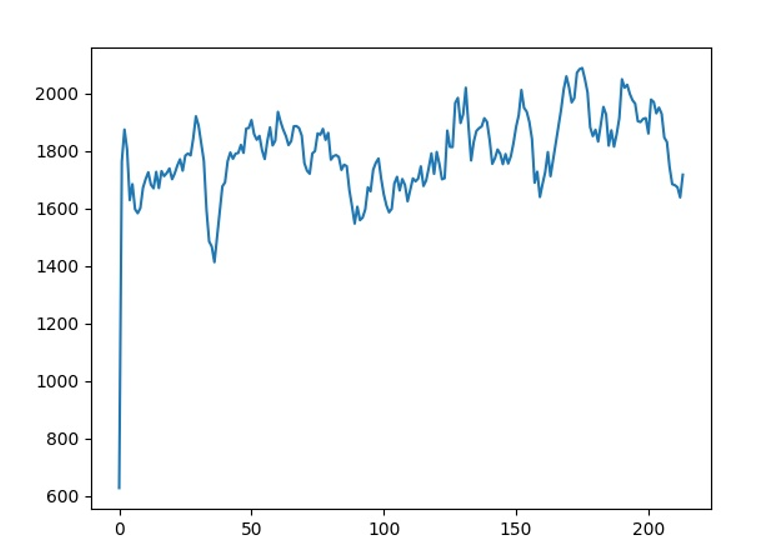
\includegraphics[width=.90\linewidth] {right_only}
    \caption{Reward plot for right only}
    \label{fig:my_label}
\end{figure}
\begin{figure}
    \centering
    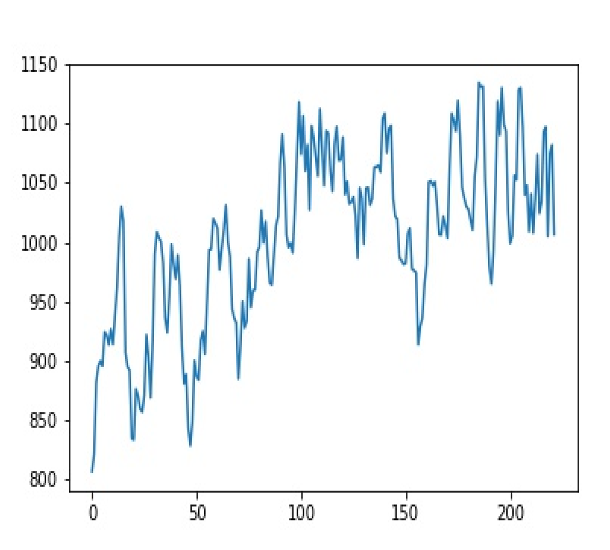
\includegraphics[width=.90\linewidth] {simple_movement}
    \caption{Reward plot for simple movement}
    \label{fig:}
\end{figure}
\begin{figure}
    \centering
    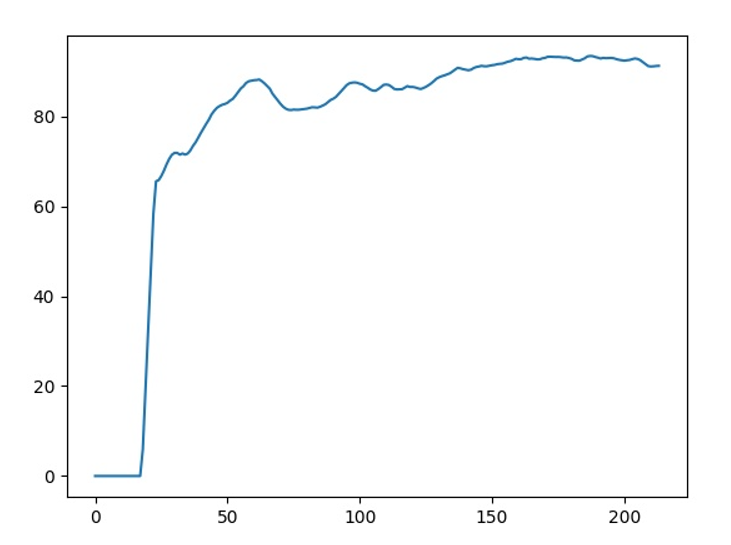
\includegraphics[width=.90\linewidth] {qplot_right}
    \caption{Q plot for right only}
    \label{fig:my_label}
\end{figure}
\begin{figure}
    \centering
    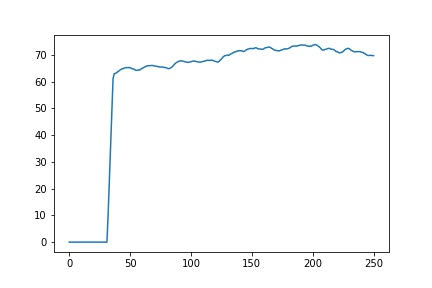
\includegraphics[width=.90\linewidth] {qplot_simple}
    \caption{Q plot for simple movement}
    \label{fig:my_label}
\end{figure}
\section{Challenges Encountered}
\begin{itemize}
  \item Environment state space given by gym had so much unnecessary information about the environment like color of the sky, trees, pipes which we had to get rid off to obtain the most useful information.
  \item There are three action sets provided by gym and as the number of actions increased, time taken by Mario to chose the next best action also increased thus leading him to die soon.
  \item It took huge time to train the agent which stunted us from training the agent more. 5000 episodes took nearly 36 hours for simple movement action space and 14 hours for right only action space.
\end{itemize}
\section{Related Works}
\cite{mnih2013playing} This paper demonstrates a convolutional neural network, trained with a variant of Q learning using experience replay, whose input is raw pixels and whose output is a value function estimating future rewards. This method has been applied on seven Atari 2600 games with no adjustment of the architecture or learning algorithm and proved to do better.
\cite{van2016deep} Authors have proposed specific adaptation to the DQN algorithm which is DDQN and show that DDQN not just reduces the observed overestimations, as hypothesized, but also leads to better performance on several games.
As stated in the abstract, we did not want to pick a complex problem statement rather a topic where we could employ as many reinforcement learning techniques as possible and understand them in-depth, we made use of the observations made in the above papers and built our agent.
\section{Conclusion}
We were successful in developing an agent using DDQN to play a Super Mario Bros game where we used right\_only and simple movement action space for world 1 level 1. As stated in the challenges, one observation that we made was as the number of actions increased, there was significant amount of delay for the agent to decide on what action to take next. This explains, why the training with right\_only action finished faster than that with simple\_movement action space. We noticed that it requires a lot of time and good hardware capacity for the training of the agent which stunted us to run it for approximately 30000 episodes for both action spaces. DDQN is efficient as the agent reached the end of the level but took longer periods of training. According to a lecture on Deep Q-Learning from Deep Mind\cite{deepmind}, Deep Q-Learning is effective in the short horizon and fast-moving games and Super Mario Bros is neither of those which could explain the delayed learning of the agent.
\\
\\
In terms of future work, we would like to increase the training of the agent in simple and expand it to complex movement action space too. We would also like to explore the next levels and include concepts like priority experience replay. 
\\
\\
Bottom line, Reinforcement Learning techniques can provide solutions to most real-life problems that do not have predefined data sets, agents can train on their own and accomplish what we want them to, after doing this project we were able to appreciate and contemplate all that has been achieved in this space and the applications and advancements that can be made are boundless.

\bibliographystyle{ieeetr}
\bibliography{ref}

\end{document}
